% arara: pdflatex
\documentclass{standalone}
\usepackage{tikz}
\usepackage{standalone}
\usetikzlibrary{positioning,arrows}
\usetikzlibrary{calc}

\begin{document}
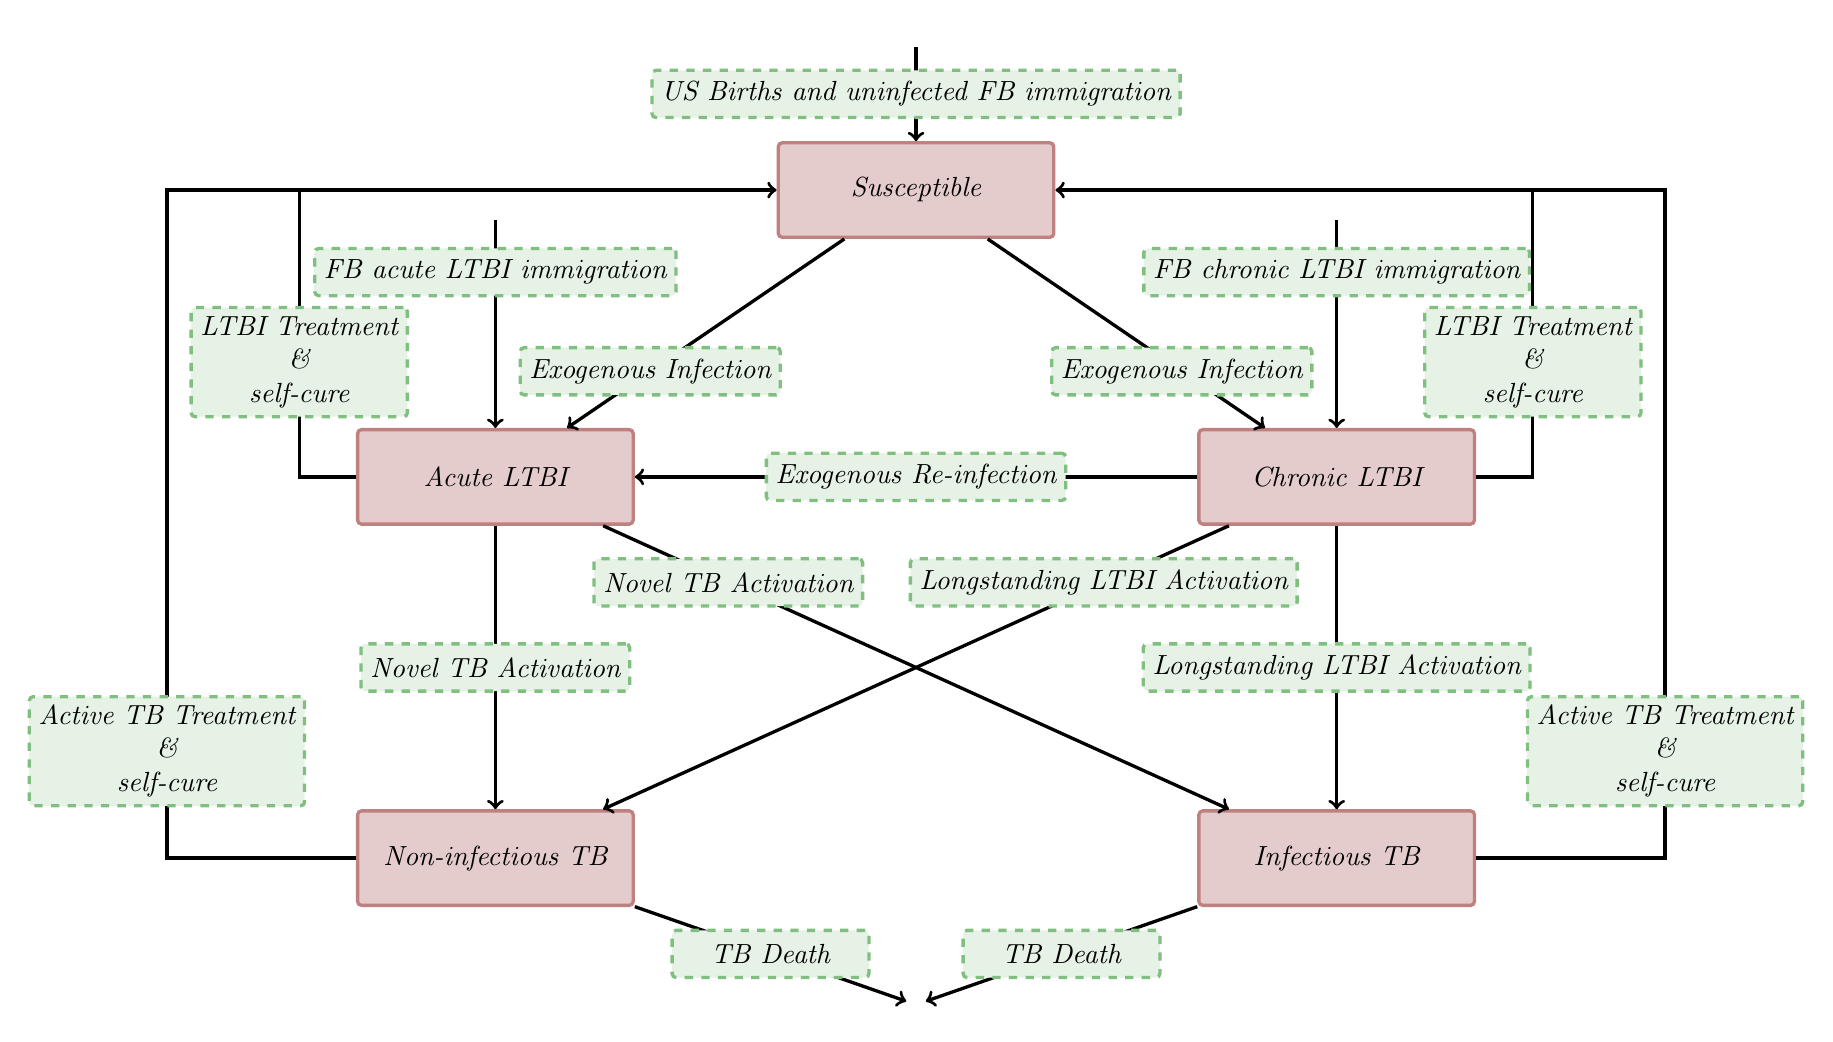
\begin{tikzpicture}
  \newdimen\dist
  \dist=1.2cm

  \tikzstyle{modelGate} = [
    % Just text!
    %% The shape:
    %rectangle, minimum height=1cm, minimum width = 3cm, rounded corners=0.5mm,
    %% The border:
    %very thick,
    %draw=blue!50!black!50,
    %% The filling:
    %top color=blue!50!black!20,
    %bottom color=blue!50!black!20,
  ];
  \tikzstyle{annotation} = [
    % Just text!
  ];
  \tikzstyle{compartment} = [
    % The shape:
    rectangle, minimum height=\dist, minimum width=3.5cm, rounded corners=0.5mm,
    % The border:
    very thick,
    draw=red!50!black!50,
    % The filling:
    top color=red!50!black!20,
    bottom color=red!50!black!20,
    % Font:
    font=\itshape
  ];
  \tikzstyle{virtualCompartment} = [
    % The shape:
    rectangle, minimum height=0.5*\dist, minimum width=2.5cm, rounded corners=0.5mm,
    % The border:
    very thick,
    draw=green!50!black!50,dashed,align=center,
    % The filling:
    top color=green!50!black!10,
    bottom color=green!50!black!10,
    % Font:
    font=\itshape
  ];
  \tikzstyle{flow} = [
    draw = black,
    very thick,
    ->
  ]
  \tikzstyle{joiningFlow} = [
    draw = black,
    very thick
  ];

  \node [modelGate] (birthAndImmigration) {};

  \node [compartment, below = \dist of birthAndImmigration] (S) {Susceptible};
  \node [compartment, below right = 2*\dist and 1.5*\dist of S] (L) {Chronic LTBI};
  \node [compartment, below left = 2*\dist and 1.5*\dist of S] (F) {Acute LTBI};

  \node [modelGate, above = 2.2*\dist of L] (FBChronicLTBIArrivals) {};
  \node [modelGate, above = 2.2*\dist of F] (FBAcuteLTBIArrivals) {};

  \node [compartment, below = 3*\dist of L] (I) {Infectious TB};
  \node [compartment, below = 3*\dist of F] (J) {Non-infectious TB};

  \node [modelGate, below = 8*\dist of S] (TBDeath) {};

  \path [flow] (birthAndImmigration) to node[virtualCompartment]
                                            {US Births and uninfected FB
                                             immigration} (S);
  \path [flow] (FBChronicLTBIArrivals) to node[virtualCompartment,pos=0.25]{FB chronic LTBI immigration} (L);
  \path [flow] (FBAcuteLTBIArrivals) to node[virtualCompartment,pos=0.25]{FB acute LTBI immigration} (F);
  \path [flow] (S) to node[virtualCompartment,pos=0.7]{Exogenous Infection} (L);
  \path [flow] (S) to node[virtualCompartment,pos=0.7]{Exogenous Infection} (F);
  \path [flow] (L) to node[virtualCompartment]{Exogenous Re-infection} (F);
  \path [flow] (L) to node[virtualCompartment]{Longstanding LTBI Activation} (I);
  \path [flow] (L) to node[virtualCompartment,pos=0.2]{Longstanding LTBI Activation} (J);
  \path [flow] (F) to node[virtualCompartment,pos=0.2]{Novel TB Activation} (I);
  \path [flow] (F) to node[virtualCompartment]{Novel TB Activation} (J);

  \newdimen\SYCoord
  \pgfextracty\SYCoord{\pgfpointanchor{S}{center}}
  \newdimen\ActiveYCoord
  \pgfextracty\ActiveYCoord{\pgfpointanchor{I}{center}}
  \newdimen\LTBIYCoord
  \pgfextracty\LTBIYCoord{\pgfpointanchor{L}{center}}

  \path [flow] (I.east) to ++(2*\dist,0) 
                        to node[virtualCompartment,pos=0.16]
                               {Active TB Treatment \\ \& \\self-cure}
                               ++(0,\SYCoord-\ActiveYCoord)
                        to (S.east);
  \path [joiningFlow] (L.east) to ++(0.6*\dist,0)
                               to node[virtualCompartment,pos=0.4]
                                      {LTBI Treatment \\ \& \\ self-cure}
                                      ++(0,\SYCoord-\LTBIYCoord);
  \path [flow] (J.west) to ++(-2*\dist,0) 
                        to node[virtualCompartment,pos=0.16]
                               {Active TB Treatment \\ \& \\ self-cure}
                               ++(0,\SYCoord-\ActiveYCoord)
                        to (S.west);
  \path [joiningFlow] (F.west) to ++(-0.6*\dist,0)
                               to node[virtualCompartment,pos=0.4]
                                      {LTBI Treatment \\ \& \\ self-cure}
                                      ++(0,\SYCoord-\LTBIYCoord);

  \path [flow] (I) to node[virtualCompartment]{TB Death} (TBDeath);
  \path [flow] (J) to node[virtualCompartment]{TB Death} (TBDeath);
\end{tikzpicture}

\end{document}
